\documentclass{../../../oss-classkick}
\tikzset{>=latex}

\begin{document}
\genheader

\gentitle{2}{THERMODYNAMICS}

\genmultidirections

\gengravity

\raggedcolumns
\begin{multicols}{2}
  \begin{enumerate}[leftmargin=18pt]
  \item Air is made up primarily of nitrogen and oxygen. In an enclosed room
    with a constant temperature, which of the following statements is
    correct concerning the nitrogen and oxygen gases?
    \begin{enumerate}[nosep,leftmargin=18pt,label=(\Alph*)]
    \item The nitrogen gas molecules have a higher average kinetic energy than
      the oxygen gas molecules.
    \item The nitrogen gas molecules have the same average kinetic energy as
      the oxygen gas molecules.
    \item The nitrogen gas molecules have a lower average kinetic energy than
      the oxygen gas molecules.
    \item More information is necessary to compare the average kinetic energies
      of the two gases.
    \end{enumerate}
    \vspace{.65in}
    
  \item Air is made up primarily of nitrogen and oxygen. In an enclosed room
    with a constant temperature, which of the following statements is correct
    concerning the nitrogen and oxygen gases?
    \begin{enumerate}[nosep,leftmargin=18pt,label=(\Alph*)]
    \item The nitrogen gas molecules have a higher velocity than the oxygen gas
      molecules.
    \item The nitrogen gas molecules have the same velocity as the oxygen gas
      molecules.
    \item The nitrogen gas molecules have a lower velocity than the oxygen gas
      molecules.
    \item It is impossible to compare the velocity of the two gases without
      knowing the temperature of the air and the percentage of nitrogen and
      oxygen in the room.
    \end{enumerate}
    \vspace{.7in}
    
  \item When using the ideal gas law, $PV=nRT$,
    \begin{enumerate}[nosep,leftmargin=18pt,label=(\Alph*)]
    \item $P$ can be gauge pressure
    \item $N$ can be in kilograms
    \item $T$ can be in degrees Celsius
    \item none of the above
    \end{enumerate}
    \vspace{.7in}

  \item For ideal gases, the ratio $PV/T $ is
    \begin{enumerate}[nosep,leftmargin=18pt,label=(\Alph*)]
    \item equal to Avogadro's number
    \item equal to Boltzmann's constant
    \item independent of the number of molecules
    \item independent of the chemical nature of the molecules
    \end{enumerate}
    \vspace{.7in}

  \item The volume of an ideal gas at constant pressure is proportional to its
    \begin{enumerate}[nosep,leftmargin=18pt,label=(\Alph*)]
    \item Fahrenheit temperature
    \item Celsius temperature
    \item Absolute temperature
    \item Molar mass
    \end{enumerate}
    \columnbreak
    
  \item In an experiment, a gas is confined in a cylinder with a movable piston.
    Force is applied to the piston to increase the pressure and change the
    volume of the gas. Each time the gas is compressed, it is allowed to
    return to a room temperature of \SI{20}{\celsius}. The data gathered from
    the experiment is shown in the table. What should be plotted on the
    vertical and horizontal axes so the slope of the graph can be used to
    determine the number of moles of gas in the cylinder?
    \begin{center}
      \begin{tabular}{ccc}
        \hline
        \textbf{Pressure} \SI{e5}{\pascal} &\hspace{.05in} &
        \textbf{Volume} \SI{e-3}{\metre^3} \\ \hline
        \num{1.0} && \num{25} \\ \hline
        \num{1.5} && \num{17} \\ \hline
        \num{1.8} && \num{14} \\ \hline
        \num{2.2} && \num{11} \\ \hline
        \num{2.6} && \num{9.6}\\ \hline
        \num{3.3} && \num{7.6}\\ \hline
      \end{tabular}
    \end{center}
    \begin{enumerate}[nosep,leftmargin=18pt,label=(\Alph*)]
    \item $P$ and $V_2$
    \item $P$ and $V$
    \item $P$ and $V^{1/2}$
    \item $P$ and $1/V$
    \end{enumerate}
    
  \item In an experiment, a sealed container with a volume of
    \SI{100}{\milli\litre} is filled with hydrogen gas. The container is heated
    to a variety of temperatures, and the pressure is measured. The data from
    the experiment is plotted in the figure. Which of the following methods
    can be used to determine additional information regarding the gas?
    Select two answers.
    \vspace{-.15in}
    \cpic{.25}{mc-q17}
    \begin{enumerate}[nosep,leftmargin=18pt,label=(\Alph*)]
    \item The slope can be used to calculate the number of atoms in the gas.
    \item The area under the graph can be used to calculate the work done by
      the gas.
    \item The vertical axis can be used to calculate the force the gas exerts
      on the container.
    \item The $x$-intercept can be used to estimate the value of absolute zero.
    \end{enumerate}
    \vspace{.7in}
    
  \item Two identical rooms are connected by an open door. The temperature in
    one room is greater than the temperature in the other. Which room contains
    the most gas molecules?
    \begin{enumerate}[nosep,leftmargin=18pt,label=(\Alph*)]
    \item The warmer room.
    \item The colder room.
    \item The number of gas molecules will be the same in both rooms.
    \item It is impossible to determine without more information.
    \end{enumerate}
    \vspace{.7in}
    \columnbreak
    
  \item On a hiking trip in the mountains, where the air temperature is cool and
    has a lower concentration of oxygen, you seal an empty water bottle.
    You return to your home near sea level where the air temperature is
    warm and has a higher concentration of oxygen. You notice that the
    sealed bottle appears partially crushed. Which of the following would
    contribute to the decrease in volume of the bottle?
    \begin{enumerate}[nosep,leftmargin=18pt,label=(\Alph*)]
    \item The change in temperature
    \item The change in atmospheric pressure
    \item The change in oxygen concentration
    \item The change in temperature, pressure, and oxygen concentration
    \end{enumerate}
    \vspace{.6in}
    
  \item The figure shows the pressure and volume of a gas at four different
    states. Which of the following correctly ranks the temperature of the gas
    at the different states?
    \begin{center}
      \vspace{-.15in}
      \pic{.3}{mc-q20}
    \end{center}
    \begin{enumerate}[nosep,leftmargin=18pt,label=(\Alph*)]
    \item $T_A>T_B>T_C>T_D$
    \item $T_B=T_C>T_A=T_D$
    \item $T_C>T_B=T_D>T_A$
    \item $T_D>T_C>T_B>T_A$
    \end{enumerate}
    \vspace{.7in}
      
  \item Which of the following is correct concerning the two processes shown
    in the figure?
    \begin{center}
      \vspace{-.15in}
      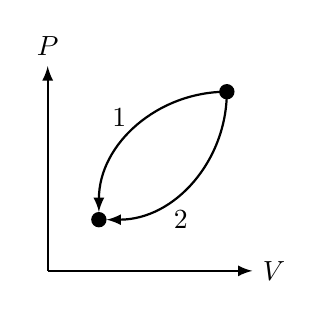
\begin{tikzpicture}[scale=1.3]
        \draw[thick,->](0,0)--(2,0) node[pos=1,right]{$V$};
        \draw[thick,->](0,0)--(0,2) node[pos=1,above]{$P$};
        \fill[black](1.75,1.75) circle(.075); %node[above]{1};
        \fill[black](0.5,0.5) circle(.075); %node[below]{2};
        \draw[thick,->](1.75,1.75) to[out=180,in=90] (.5,.575);
        \draw[thick,->](1.75,1.75) to[out=270,in=0] (.575,.5);
        \node at (1.3,.5) {2}; %[midway,above]{1};
        \node at (.7,1.5) {1}; %[midway,above]{1};
      \end{tikzpicture}
    \end{center}
    \begin{enumerate}[nosep,leftmargin=18pt,label=(\Alph*)]
    \item $\Delta U_1 = \Delta U_2$ and $W_1= W_2$
    \item $\Delta U_1 = \Delta U_2$ and $W_1>W_2$
    \item $\Delta U_1 > \Delta U_2$ and $W_1=W_2$
    \item $\Delta U_1 > \Delta U_2$ and $W_1\geq W_2$
    \end{enumerate}
    \vspace{.7in}
    
  \item The figure shows four samples of gas being taken through four
    different processes. Process 1 is adiabatic. In which process is heat being
    transferred to the gas sample from the environment?
    \vspace{-.15in}
    \cpic{.35}{mc-q22}
    \begin{enumerate}[nosep,leftmargin=18pt,label=(\Alph*)]
    \item 1
    \item 2
    \item 3
    \item 4
    \end{enumerate}
    \columnbreak
    
  \item Two sealed cylinders holding different gases are placed one on top of
    the other so heat can flow between them. Cylinder A is filled with
    hydrogen. Cylinder B is filled with helium moving with an average speed
    that is half that of the hydrogen atoms. Helium atoms have four times the
    mass of hydrogen atoms. Which of the following best describes the transfer
    of heat between the two containers by conduction?
    \begin{enumerate}[nosep,leftmargin=18pt,label=(\Alph*)]
    \item Net heat flows from cylinder A to cylinder B, because heat flows from
      higher kinetic energy atoms to lower kinetic energy atoms.
    \item Net heat flows from cylinder B to cylinder A, because heat flows from
      higher kinetic energy atoms to lower kinetic energy atoms.
    \item There is no net heat transfer between the two cylinders, because both
      gases have the same average atomic kinetic energy.
    \item There is no net heat transfer between the two cylinders, because heat
      conduction requires the movement of atoms between the cylinder, and the
      cylinders are sealed.
    \end{enumerate}
  \end{enumerate}
  \vspace{.7in}
  
  \textbf{Questions \ref{q-start} and \ref{q-end}}

  A gas beginning at point O on the graph can be taken along four paths to
  different ending conditions.
  \vspace{-.15in}
  \cpic{.35}{mc-q24-25}
  \begin{enumerate}[leftmargin=18pt,resume]

  \item Which of the following are the same for processes 2 and 3?
    \emph{Select two answers.}
    \label{q-start}
    \begin{enumerate}[nosep,leftmargin=18pt,label=(\Alph*)]
    \item $Q$
    \item $\Delta T$
    \item $\Delta U$
    \item $W$
    \end{enumerate}
    
  \item Along which of the paths is the most thermal energy removed from the
    gas?
    \label{q-end}
    \begin{enumerate}[nosep,leftmargin=18pt,label=(\Alph*)]
      \item\num{1}
      \item\num{2}
      \item\num{3}
      \item\num{4}
    \end{enumerate}
    
  \item The graph shows the distribution of speeds for one mole of hydrogen at
    temperature $T$, pressure $P$, and volume $V$. How would the graph change
    if the sample was changed from one mole hydrogen to one mole of argon at
    the same temperature, pressure, and volume?
    \begin{center}
      \vspace{-.15in}
      \pic{.35}{mc-q26}
    \end{center}
    \begin{enumerate}[nosep,leftmargin=18pt,label=(\Alph*)]
    \item The peak will shift to the left
    \item The peak will shift upward and to the left
    \item The peak will shift to the right
    \item The peak will shift downward and to the right
    \end{enumerate}
    \columnbreak

  \item The graph shows the pressure and volume of a gas being taken from state
    \#1 to state \#2. Which of the following correctly indicates the sign of
    the work done by the gas, and the change in temperature of the gas?
    \begin{center}
      \vspace{-.15in}
      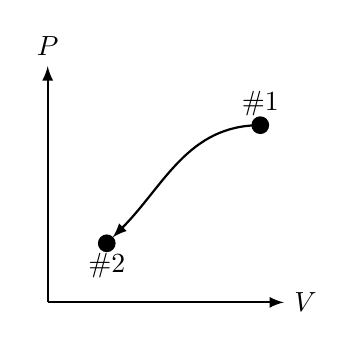
\begin{tikzpicture}[scale=1.5]
        \draw[thick,->](0,0)--(2,0)
        node[pos=1,right]{$V$};
        \draw[thick,->](0,0)--(0,2) node[pos=1,above]{$P$};
        \fill[black](1.8,1.5) circle(.075) node[above]{\#1};
        \fill[black](0.5,0.5) circle(.075) node[below]{\#2};
        \draw[thick,->](1.8,1.5) to[out=180,in=45] (.55,.55);
      \end{tikzpicture}

      \begin{tabular}{ccc}
        & \textbf{Work done} & $\Delta$ \textbf{Temperature}\\ \hline
        (A) & $+$ & $+$ \\
        (B) & $+$ & $-$ \\
        (C) & $-$ & $+$ \\
        (D) & $-$ & $-$
      \end{tabular}
    \end{center}
    \vspace{.7in}
    
  \item What is the volume of one mole of ideal gas at \SI{300}{K} and at
    standard atmospheric pressure?
    \begin{enumerate}[nosep,leftmargin=18pt,label=(\Alph*)]
    \item\SI{23.2}{\litre}
    \item\SI{24.1}{\litre}
    \item\SI{24.6}{\litre}
    \item\SI{25.7}{\litre}
    \end{enumerate}
    
  \item A fixed mass of oxygen (O\textsubscript{2}, molecular mass
    \SI{32}{g/mol}) is contained in a cylinder whose volume is \num{2.80}
    liters. The pressure is \SI{148}{atm} when the temperature is
    \SI{23}{\celsius}. Find the mass of oxygen in the cylinder.
    \begin{enumerate}[nosep,leftmargin=18pt,label=(\Alph*)]
    \item\SI{20}{\gram}
    \item\SI{80}{\gram}
    \item\SI{140}{\gram}
    \item\SI{280}{\gram}
    \item\SI{546}{\gram}
    \end{enumerate}
    \columnbreak
    
  \item A tire is filled with air at \SI{15}{\celsius} to a gauge pressure of
    \SI{2.2e5}{\pascal}. If the tire reaches a temperature of \SI{38}{\celsius},
    what will the new gauge pressure be inside it?
    \begin{enumerate}[nosep,leftmargin=18pt,label=(\Alph*)]
    \item\SI{2.4e2}{\pascal}
    \item\SI{3.4e3}{\pascal}
    \item\SI{2.4e5}{\pascal}
    \item\SI{6.0e7}{\pascal}
    \item\SI{8.0e9}{\pascal}
    \end{enumerate}

  \item A fixed mass of an ideal gas having a volume of \SI{2500}{cm^3} at
    \SI{20}{\celsius} and absolute pressure of \SI{65}{atm} expands until its
    volume is \SI{4000}{cm^3} and its absolute pressure is \SI{45}{atm}. Find
    its new temperature.
    \begin{enumerate}[nosep,leftmargin=18pt,label=(\Alph*)]
    \item\SI{20}{\celsius}
    \item\SI{42.3}{\celsius}
    \item\SI{51.6}{\celsius}
    \item\SI{61.8}{\celsius}
    \item\SI{80}{\celsius}
    \end{enumerate}

  \item A fixed mass of an ideal gas is in a container with a constant volume.
    By what factor will the pressure change if the absolute temperature is
    tripled?
    \begin{enumerate}[nosep,leftmargin=18pt,label=(\Alph*)]
    \item 1/9
    \item 1/3
    \item 3
    \item 9
    \end{enumerate}

  \item If the pressure of gas is doubled and the temperature is constant, then
    the volume is what factor times the original?
    \begin{enumerate}[nosep,leftmargin=18pt,label=(\Alph*)]
    \item 2
    \item 1/2
    \item 1/4
    \item 4
    \end{enumerate}
   

%  \item An ideal gas in a container has a pressure of \SI{2.50}{atm} and a
%    volume of \SI{1}{m^3} at a temperature of \SI{30}{\celsius}. How many moles
%    of gas are in the container?
%    \begin{enumerate}[nosep,leftmargin=18pt,label=(\Alph*)]
%    \item\SI{20}{moles}
%    \item\SI{45}{moles}
%    \item\SI{62}{moles}
%    \item\SI{83}{moles}
%    \item\SI{100}{moles}
%    \end{enumerate}

  \end{enumerate}
\end{multicols}

%\newpage
%\genanswersheet{2}{Fluid Mechanics \& Thermodynamics}
%
%\begin{center}
%  \begin{minipage}[t]{.2\textwidth}
%    \vspace{.2in}
%    \bgroup
%    \begin{tabular}{>{\centering}m{1.3cm} >{\centering}m{1.7cm}}
%      No. & Answer
%    \end{tabular}\\
%    \def\arraystretch{1.5}
%    \begin{tabular}{|>{\centering}m{1.3cm}|>{\centering}m{1.7cm}|}
%      \hline
%      1 & \\ \hline
%      2 & \\ \hline
%      3 & \\ \hline
%      4 & \\ \hline
%      5 & \\ \hline
%      6 & \\ \hline
%      7 & \\ \hline
%      8 & \\ \hline
%      9 & \\ \hline
%      10 & \\ \hline
%      11 & \\ \hline
%      12 & \\ \hline
%      13 & \\ \hline
%      14 & \\ \hline
%      15 & \\ \hline
%      16 & \\ \hline
%      17 & \\ \hline
%      18 & \\ \hline
%      19 & \\ \hline
%      20 & \\ \hline
%      21 & \\ \hline
%      22 & \\ \hline
%      23 & \\ \hline
%      24 & \\ \hline
%      25 & \\ \hline
%    \end{tabular}
%    \egroup
%  \end{minipage}
%  \hspace{.5in}
%  \begin{minipage}[t]{.2\textwidth}
%    \vspace{.2in}
%    \bgroup
%    \begin{tabular}{>{\centering}m{1.3cm} >{\centering}m{1.7cm}}
%      No. & Answer
%    \end{tabular}\\
%    \def\arraystretch{1.5}
%    \begin{tabular}{|>{\centering}m{1.3cm}|>{\centering}m{1.7cm}|}
%      \hline
%      26 & \\ \hline
%      27 & \\ \hline
%      28 & \\ \hline
%      29 & \\ \hline
%      30 & \\ \hline
%      31 & \\ \hline
%      32 & \\ \hline
%      33 & \\ \hline
%      34 & \\ \hline
%      35 & \\ \hline
%      36 & \\ \hline
%      37 & \\ \hline
%    \end{tabular}
%    \egroup
%  \end{minipage}
%\end{center}
\newpage

\genfreetitle{2}{Thermodynamics of Gases}{4}

\genfreedirections

% THIS TAKEN FROM THE 2001 AP PHYSICS B EXAM FREE-RESPPONSE QUESTION #6
\begin{center}
  \pic{.8}{gases}\\
  \underline{Note:} Figure not drawn to scale.
\end{center}
\begin{enumerate}[leftmargin=15pt]
\item A cylinder is fitted with a freely movable piston of area
  \SI{1.20e-2}{\metre^2} and negligible mass. The cylinder below the piston is
  filled with a gas. At state 1, the gas has volume \SI{1.50e-3}{\metre^3},
  pressure \SI{1.02e5}{\pascal}, and the cylinder is in contact with a water
  bath at a temperature of \SI{0}{\celsius}. The gas is then taken through the
  following four-step process.
  \begin{itemize}
  \item A 2.50 kg metal block is placed on top of the piston, compressing the
    gas to state 2, with the gas still at \SI{0}{\celsius}.
  \item The cylinder is then brought in contact with a boiling water bath,
    raising the gas temperature to \SI{100}{\celsius} at state 3.
  \item The metal block is removed and the gas expands to state 4 still at
    \SI{100}{\celsius}.
  \item Finally, the cylinder is again placed in contact with the water bath at
    \SI{0}{\celsius}, returning the system to state 1.
  \end{itemize}
  \begin{enumerate}
  \item Determine the pressure of the gas in state 2.
  \item Determine the volume of the gas in state 2.
  \item Indicate below whether the process from state 2 to state 3 is
    isothermal, isobaric, or adiabatic. Explain your reasoning.

    \vspace{.1in}
    \underline{\hspace{.3in}} Isothermal\hspace{.5in}
    \underline{\hspace{.3in}} Isobaric\hspace{.5in}
    \underline{\hspace{.3in}} Adiabatic
    \vspace{1in}
    
  \item Is the process from state 4 to state 1 isobaric? Explain your
    reasoning.

    \vspace{.1in}\underline{\hspace{.3in}}Yes\hspace{.5in}
    \underline{\hspace{.3in}} No
    \vspace{1in}

  \item Determine the volume of the gas in state 4.\vspace{.35in}
  \end{enumerate}
  \newpage
  
  % THIS TAKEN FROM THE 2005 AP PHYSICS B EXAM FREE-RESPPONSE QUESTION #6
  \cpic{.2}{piston}
\item An experiment is performed to determine the number $n$ of moles of an
  ideal gas in the cylinder shown above. The cylinder is fitted with a movable,
  frictionless piston of area $A$. The piston is in equilibrium and is supported
  by the pressure of the gas. The gas is heated while its pressure $P$ remains
  constant. Measurements are made of the temperature $T$ of the gas and the
  height $H$ of the bottom of the piston above the base of the cylinder and are
  recorded in the table below. Assume that the thermal expansion of the
  apparatus can be ignored.
  \begin{center}
    \begin{tabular}{|c|c|}
      \hline
      $T$ (\si{\kelvin}) & $H$ (\si{\metre}) \\ \hline\hline
      300 & 1.11 \\
      325 & 1.19 \\
      355 & 1.29 \\
      375 & 1.37 \\
      405 & 1.47 \\
      \hline
    \end{tabular}
  \end{center}
  \begin{enumerate}
  \item Write a relationship between the quantities $T$ and $H$, in terms of
    the given quantities and fundamental constants, that will allow you to
    determine $n$.
  \item Plot the data on the axes below so that you will be able to determine
    $n$ from the relationship in part (a). Label the axes with appropriate
    numbers to show the scale.
    \begin{center}
      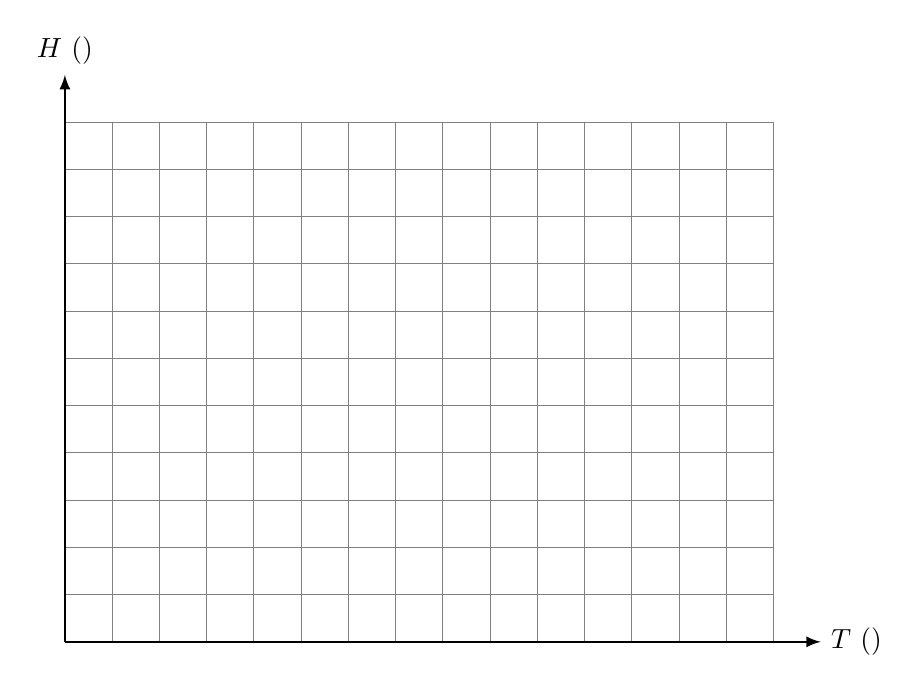
\begin{tikzpicture}[scale=.6]
        \draw[thin,gray](0,0) grid(15,11);
        \draw[thick,->](0,0)--(16,0) node[right]{$T$ (\si{\kelvin})};
        \draw[thick,->](0,0)--(0,12) node[above]{$H$ (\si{\metre})};
      \end{tikzpicture}
    \end{center}
  \item Using your graph and the values $A=\SI{0.027}{\metre\squared}$ and
    $P=\SI{1.}{atm}$, determine the experimental value of $n$.
    \vspace{1in}
  \end{enumerate}


%\item An air bubble is released from the bottom of a swimming pool and ascends
%  to the surface.
%  \begin{enumerate}[leftmargin=18pt]
%  \item In a clear, coherent, paragraph-length response, describe any changes
%    in the bubble size and describe the motion of the bubble
%    as it ascends to the surface. Explain the factors that affect the size
%    of the bubble and the bubble's motion. Include a description of
%    any forces acting on the bubble from the time it is at the bottom of
%    the pool until it reaches the surface.
%    \vspace{1.75in}
%    
%  \item Draw a diagram of all the forces acting on the bubble. Make sure
%    the forces are in correct proportion.
%    \vspace{1.75in}
%
%  \item The bubble does not collapse under the pressure of the water.
%    Explain how the behavior of the gas atoms keep the bubble from
%    collapsing.
%    \newpage
%    
%  \item The bubble has an initial volume of $V_D$ , begins at a depth of $D$
%    below the surface of the water, and reaches the surface where the
%    pressure is $P_S$ . The density of the water is $r$.
%    \begin{enumerate}
%    \item  Derive an expression for the initial pressure ($P_D$) in the bubble
%      in terms of the given quantities and known constants.
%    \item Assume the air temperature in the bubble remains the same as
%      it rises. Derive an expression for the volume ($V_S$) of the bubble
%      when it reaches the surface.
%    \end{enumerate}
%    \vspace{2in}
%    
%  \item Now assume that the bubble rises quickly to the surface, and that
%    there is negligible thermal energy transfer between the bubble and the
%    swimming pool. Base your answers on this assumption.
%    \begin{enumerate}
%    \item Sketch the process on the $PV$ diagram. Indicate on the axis the
%      initial and final pressures and volumes.
%    \item How does the value $P_S$--$V_S$ compare to the value $P_D$--$V_D$?
%
%      \vspace{
%      %__Greater than P D V D __Equal to P D V D __Less than P D V D
%      Justify your answer.
%    \end{enumerate}
%    \vspace{1.75in}
%    
%  \item The bubble passes through higher temperature water as it nears the
%    sun-warmed surface of the pool. Unexpectedly, this allows a
%    sizable amount of thermal energy to transfer from the water to the
%    bubble as it rises. How does this affect the final volume of the
%    bubble? Justify your answer.
%  \end{enumerate}
  \newpage
  
  \cpic{.35}{process1}
\item A sample containing three moles of an ideal gas is taken through a series
  of equilibrium states, as represented by the closed path $ABCDA$ in the
  diagram above.
  \begin{enumerate}
  \item
    \begin{enumerate}
    \item Rank the temperatures at the 4 labeled points from least to greatest,
      using 1 for the lowest temperature. If two or more points have the same
      temperature, give them the same ranking.

      \vspace{.1in}
      \underline{\hspace{.3in}} A\hspace{.2in}
      \underline{\hspace{.3in}} B\hspace{.2in}
      \underline{\hspace{.3in}} C\hspace{.2in}
      \underline{\hspace{.3in}} D
      
    \item Determine the temperature $T_D$ at point $D$ in terms of $P_0$, $V_0$,
      and fundamental constants, as appropriate.
      \vspace{\stretch1}
    \end{enumerate}
    
  \item Indicate all segments of the path $ABCDA$, if any, for which the work
    done by the gas is positive. If the work done by the gas is not positive
    for any of the segments, then check ``None''. Justify your answer.

    \vspace{.1in}
    \underline{\hspace{.3in}} AB\hspace{.2in}
    \underline{\hspace{.3in}} BC\hspace{.2in}
    \underline{\hspace{.3in}} CD\hspace{.2in}
    \underline{\hspace{.3in}} DA\hspace{.2in}
    \underline{\hspace{.3in}} None
    \vspace{\stretch1}
    
  \item In process $AB$, is the energy transferred to the gas by heating
    positive, negative, or zero? Justify your answer.
    
    \vspace{.1in}
    \underline{\hspace{.3in}} Positive\hspace{.2in}
    \underline{\hspace{.3in}} Negative\hspace{.2in}
    \underline{\hspace{.3in}} Zero    
    \vspace{\stretch1}

  \item Derive an expression for the net work done on the gas during the entire
    process $ABCDA$. Express your answer in terms of $P_0$, $V_0$, and
    fundamental constants, as appropriate.
    \vspace{\stretch2}
  \end{enumerate}
  \newpage
  
%\item A mole of ideal gas is enclosed in a cylinder with a movable piston
%  with a cross-sectional area of \SI{1e-2}{m^2}. The gas is taken through a
%  thermodynamic process, as shown in the figure.
%  \begin{center}
%    \pic{.4}{fr-q3a}
%  \end{center}
%  \begin{enumerate}
%  \item Calculate the temperature of the gas at state A, and describe the
%    microscopic property of the gas that is related to the
%    temperature.
%    \vspace{1in}
%  \item Calculate the force of the gas on the piston at state A, and
%    explain how the atoms of the gas exert this force on the piston.
%    \vspace{1in}
%  \item Predict qualitatively the change in the internal energy of the gas
%    as it is taken from state B to state C. Justify your prediction.
%    \vspace{1in}
%  \item Is heat transferred to or from the gas as it is taken from state B to
%    state C? Justify your answer.
%    \newpage
%
%  \item Discuss any entropy changes in the gas as it is taken from state B
%    to state C. Justify your answer.
%    \vspace{1in}
%  \item Calculate the change in the total kinetic energy of the gas atoms
%    as the gas is taken from state C to state A.
%    \vspace{1in}
%  \item On the axis provided, sketch and label the distribution of the speeds
%    of the atoms in the gas for states A and B.
%    \begin{center}
%      \begin{tikzpicture}[scale=4]
%        \draw[very thick,->](0,0)--(3,0)
%        node[midway,below]{speed};
%        \draw[very thick,->](0,0)--(0,2)
%        node[midway,above,sloped]{number of atoms};
%      \end{tikzpicture}
%    \end{center}
%  \end{enumerate}

\item You wish to determine the relationship between gas pressure and
  temperature.
  \begin{enumerate}
  \item List the items you would use to perform this investigation.
    \vspace{1.5in}
    
  \item Draw a simple picture of the lab setup, and outline the experimental
    procedure you would use to gather the necessary data. Indicate the
    measurements to be taken and how the measurement will be used to obtain the
    data needed. Make sure your outline contains sufficient detail so that
    another student could follow your procedure.
    \vspace{1.75in}
  \item On the axis, sketch the line or curve that you predict will represent
    the results of the data gathered in this experiment.
    \begin{center}
      \begin{tikzpicture}[scale=1.75]
        \draw[very thick,->](0,0)--(2,0) node[right]{$P$};
        \draw[very thick,->](0,0)--(0,2) node[above]{$T$};
      \end{tikzpicture}
    \end{center}
    
  \item Explain how you could use your results to estimate the value of
    absolute zero.
  \end{enumerate}
  \newpage
  
  You are given the following set of data acquired in a gas laboratory
  experiment and asked to determine the relationship between pressures and
  volume for the gas.
  \vspace{-.1in}
  \cpic{.36}{fr-q4}
  \begin{enumerate}[resume]
  \item Which subset of the data would be most useful in creating a graph to
    determine the relationship between gas pressure and volume? Explain why the
    trials you selected are the most useful.
    \vspace{.5in}
    
  \item Plot the subset of data you chose on the graph, being sure to label the
    axes. Draw a line or curve that best represents the relationship between
    the variables.
    \begin{center}
      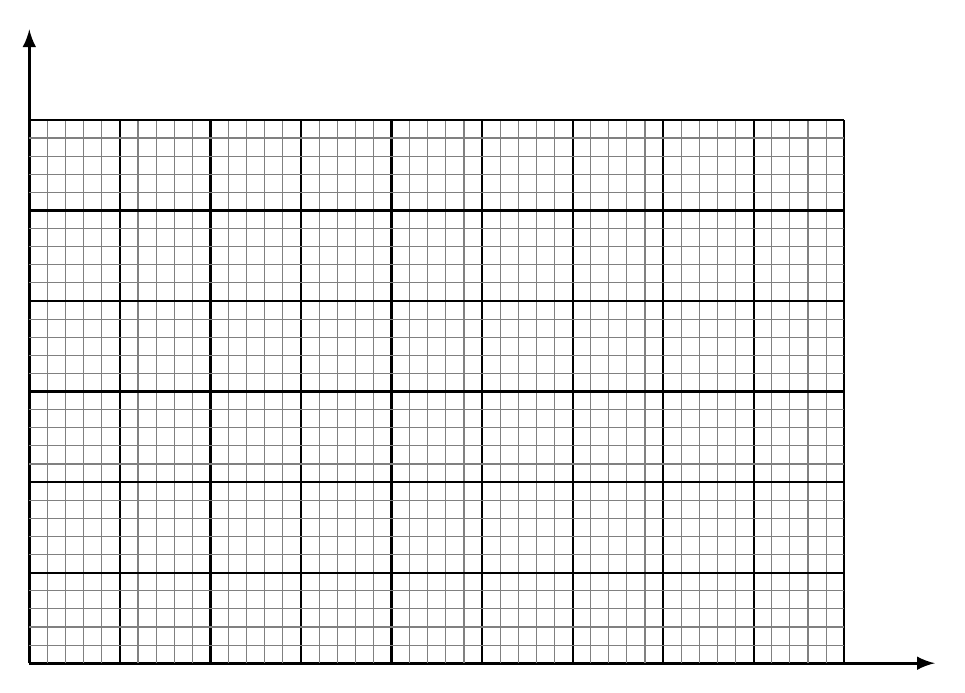
\begin{tikzpicture}[scale=2.3]
        \draw[very thick,->](0,0)--(5,0);
        \draw[very thick,->](0,0)--(0,3.5);
        \foreach \x in {.1,.2,...,4.5} \draw[gray](\x,0)--(\x,3);
        \foreach \xx in {.5,1,...,4.5} \draw[thick](\xx,0)--(\xx,3);
        \foreach \y in {.1,.2,...,3}   \draw[gray](0,\y)--(4.5,\y);
        \foreach \yy in {.5,1,...,3}   \draw[thick](0,\yy)--(4.5,\yy);
      \end{tikzpicture}
    \end{center}
  \item What can you conclude from your line or curve about the relationship
    between volume and pressure?
  \end{enumerate}
\end{enumerate}
\end{document}
